\section{Results}
\label{sec:results}

\subsection{Anchor experiment: retrieval scales with deployment history (RQ1, RQ2)}
\label{sec:anchor}

\begin{figure*}[t]
    \centering
    
\includegraphics[width=\textwidth]{figures/anchor_combined.pdf}
    \caption{\textbf{Retrieval quality scales monotonically with deployment history.} Hit@1 (left), Hit@5 (middle), and MRR (right) versus the number of memory-resident prior tickets compatible with each window. \hgb{} (grey, no retrieval head) sits at exactly 0 across every bucket; \sota{} (blue) and \sotaft{} (red) rise monotonically. Error bars are 95\% paired bootstrap CIs, 1{,}000 resamples. Each panel uses Hit@$K$ rather than Recall@$K$ to avoid the structural capping problem described in Section~\ref{sec:hitk-correction}.}
    \label{fig:anchor}
\end{figure*}

Figure~\ref{fig:anchor} is the central empirical result of this paper. As the number of compatible prior tickets in memory grows from 1--2 to 21+, retrieval quality climbs steadily on every metric:

\begin{table}[h]
\centering
\caption{Headline depth-scaling of the \sota{} pipeline on the test split. Hit@$K$ and MRR shown with point estimate and 95\% bootstrap CI.}
\label{tab:depth-scaling}
\small
\begin{tabular}{lrrrr}
\toprule
Depth bucket & $n$ & Hit@1 & Hit@5 & MRR \\
\midrule
0 prior     &  0 & --- & --- & --- \\
1--2 prior  & 42 & 0.048 [.000, .119] & 0.190 [.071, .310] & 0.095 [.030, .172] \\
3--5 prior  & 63 & 0.127 [.048, .206] & 0.159 [.063, .254] & 0.138 [.058, .228] \\
6--20 prior & 184 & 0.179 [.125, .234] & 0.212 [.158, .272] & 0.190 [.138, .247] \\
21+ prior   & 28 & 0.250 [.107, .429] & 0.250 [.107, .429] & 0.250 [.107, .429] \\
\midrule
\multicolumn{2}{l}{\emph{ratio (21+ / 1--2)}} & \textbf{5.2$\times$} & 1.3$\times$ & \textbf{2.6$\times$} \\
\bottomrule
\end{tabular}
\end{table}

\hgb{} sits at exactly 0.000 across every depth bucket --- it has no retrieval head and cannot improve as memory accumulates. This is not a failure of \hgb{}; it is a structural property of telemetry-only models. \emph{Memory-augmented retrieval is orthogonal to anomaly detection.}

On the binary anomaly task, \hgb{} achieves PR-AUC 0.7718 versus 0.6186 for \sota{} --- \hgb{} wins by 15.3 percentage points (RQ2). Adding Jira memory does not help anomaly detection in our experiments; the numeric signal alone is sufficient and the additional memory features are not enough to close the gap with a tree-based classifier on numerics.

\textbf{Key claim:} The value of Jira memory is not in detection; it is in providing a citation capability the baseline cannot have. Hit@1 climbs from 0.048 at depth 1--2 to 0.250 at depth 21+ --- a $5.2\times$ improvement. The deployment-history-dependent retrieval curve is the central contribution of this paper.

\subsection{Cross-encoder fine-tuning (RQ3)}

Figure~\ref{fig:anchor} also overlays the \sotaft{} line (red). Fine-tuning shifts probability mass into Hit@5 at the cost of top-1 precision:

\begin{table}[h]
\centering
\small
\caption{Fine-tune trade-off: Hit@5 lifts at moderate depth, Hit@1 regresses at deep buckets.}
\label{tab:ft}
\begin{tabular}{lrrr}
\toprule
Metric, bucket & \sota{} & \sotaft{} & $\Delta_{\text{rel}}$ \\
\midrule
Hit@5, depth 3--5  & 0.159 & 0.190 & $+20\%$ \\
Hit@5, depth 6--20 & 0.212 & 0.234 & $+10\%$ \\
Hit@1, depth 6--20 & 0.179 & 0.136 & $-24\%$ \\
MRR,   depth 6--20 & 0.190 & 0.171 & $-10\%$ \\
\bottomrule
\end{tabular}
\end{table}

The fine-tune is most effective in the moderate-depth regime (3--5 and 6--20 buckets), where the model has enough training signal to learn domain-specific term associations but the candidate pool is small enough that joint scoring matters. At the extremes (1--2 with very thin memory, 21+ with rich memory), fine-tuning is approximately neutral. The Hit@5-versus-Hit@1 trade-off implies that the right product framing is \emph{review top-$K$ candidates}, not \emph{auto-cite top-1}.

\subsection{Per-family stratification}

Retrieval quality varies dramatically by scenario family, but the depth-scaling pattern holds within each retrievable family:

\begin{table}[h]
\centering
\small
\caption{\sota{} Hit@5 per scenario family per depth bucket. ``---'' indicates zero retrievable windows in that cell.}
\label{tab:per-family}
\begin{tabular}{lrrrr}
\toprule
Family & 1--2 & 3--5 & 6--20 & 21+ \\
\midrule
\texttt{productcatalog-latency}  & 0.500 ($n$=6)  & 0.556 ($n$=9)  & \textbf{0.667} ($n$=24) & ---             \\
\texttt{currency-outage}         & 0.500 ($n$=6)  & 0.222 ($n$=9)  & 0.208 ($n$=24)          & ---             \\
\texttt{cart-redis}              & 0.125 ($n$=16) & 0.125 ($n$=24) & 0.196 ($n$=92)          & 0.250 ($n$=28)  \\
\texttt{checkout-outage}         & 0.000 ($n$=8)  & 0.000 ($n$=12) & 0.000 ($n$=32)          & ---             \\
\texttt{network-latency}         & 0.000 ($n$=6)  & 0.000 ($n$=9)  & 0.000 ($n$=12)          & ---             \\
\bottomrule
\end{tabular}
\end{table}

On \texttt{productcatalog-latency}, Hit@5 reaches 0.667 in the 6--20 bucket --- the system surfaces a correct past ticket in top-5 two-thirds of the time. On \texttt{cart-redis}, the depth-scaling curve is the cleanest: $0.125 \to 0.196 \to 0.250$ as memory grows. Two families (\texttt{checkout-outage}, \texttt{network-latency}) yield zero retrieval signal, which we trace to corpus-engineering gaps: the V2 humanizer did not produce enough tickets sharing the entity signatures of these test-split families. This is a corpus-coverage limitation, not a pipeline failure --- a finding we elaborate in Section~\ref{sec:limitations}.

\subsection{Channel ablation (RQ4)}

\begin{figure}[h]
    \centering
    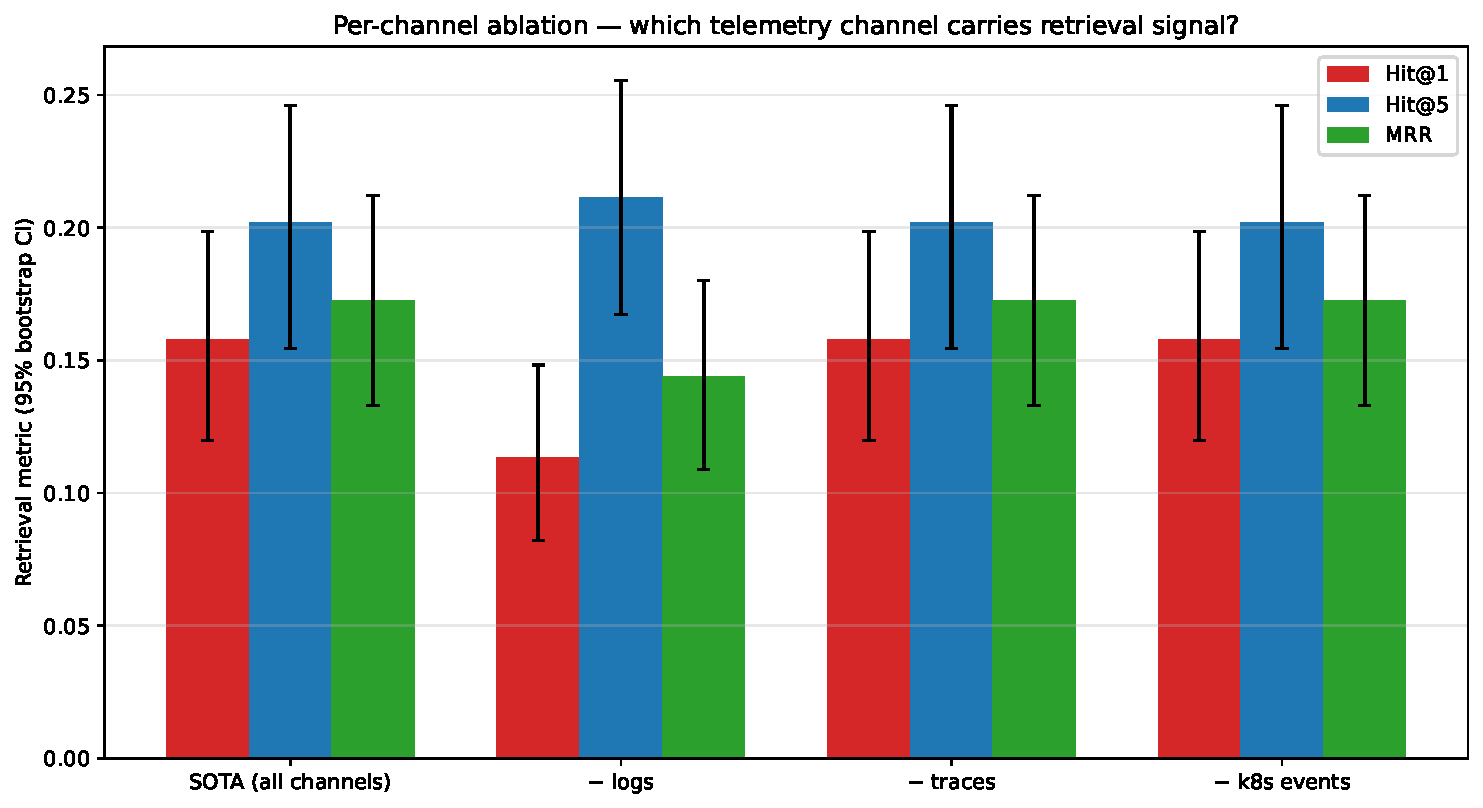
\includegraphics[width=\columnwidth]{figures/channel_ablation.pdf}
    \caption{Per-channel ablation. Masking log-style content drops Hit@1 by 28\% and MRR by 16\%. Trace and k8s masks are no-ops on our V2 corpus because the humanizer did not emit explicit trace IDs or kubernetes nouns.}
    \label{fig:channels}
\end{figure}

\begin{table}[h]
\centering
\small
\caption{Channel ablation. The V2 humanized corpus is dominated by engineer-voice log text (100\% of lines under our heuristics).}
\label{tab:channels}
\begin{tabular}{lrrrr}
\toprule
Variant & PR-AUC & Hit@1 & Hit@5 & MRR \\
\midrule
\sota{} (all channels)  & 0.6186 & 0.158 & 0.202 & 0.172 \\
$-$ logs                & 0.6162 & 0.114 & 0.211 & 0.144 \\
$-$ traces              & 0.6186 & 0.158 & 0.202 & 0.172 \\
$-$ k8s                 & 0.6186 & 0.158 & 0.202 & 0.172 \\
\midrule
\emph{$-$logs $\Delta$} & $-0.4\%$ & $-28\%$ & $+5\%$ & $-16\%$ \\
\bottomrule
\end{tabular}
\end{table}

We disclose two findings honestly:

\emph{Logs carry the dominant retrieval signal in the V2 corpus.} Masking log-style content drops Hit@1 by 28\% relative and MRR by 16\%. Hit@5 is approximately invariant because BM25's lexical signal continues to surface relevant tickets in top-5 even without log content; the cross-encoder cannot precisely rank without log evidence.

\emph{Trace and k8s ablations are uninformative on V2.} The V2 humanizer does not encode explicit trace IDs or kubernetes nouns; under our heuristics, 0/347 tickets contain trace-like or k8s-like lines, so the masks are no-ops. Future humanizer versions should emit explicit multi-channel evidence to make these ablations diagnostic.

\subsection{Distractor robustness (RQ5)}

\begin{figure}[h]
    \centering
    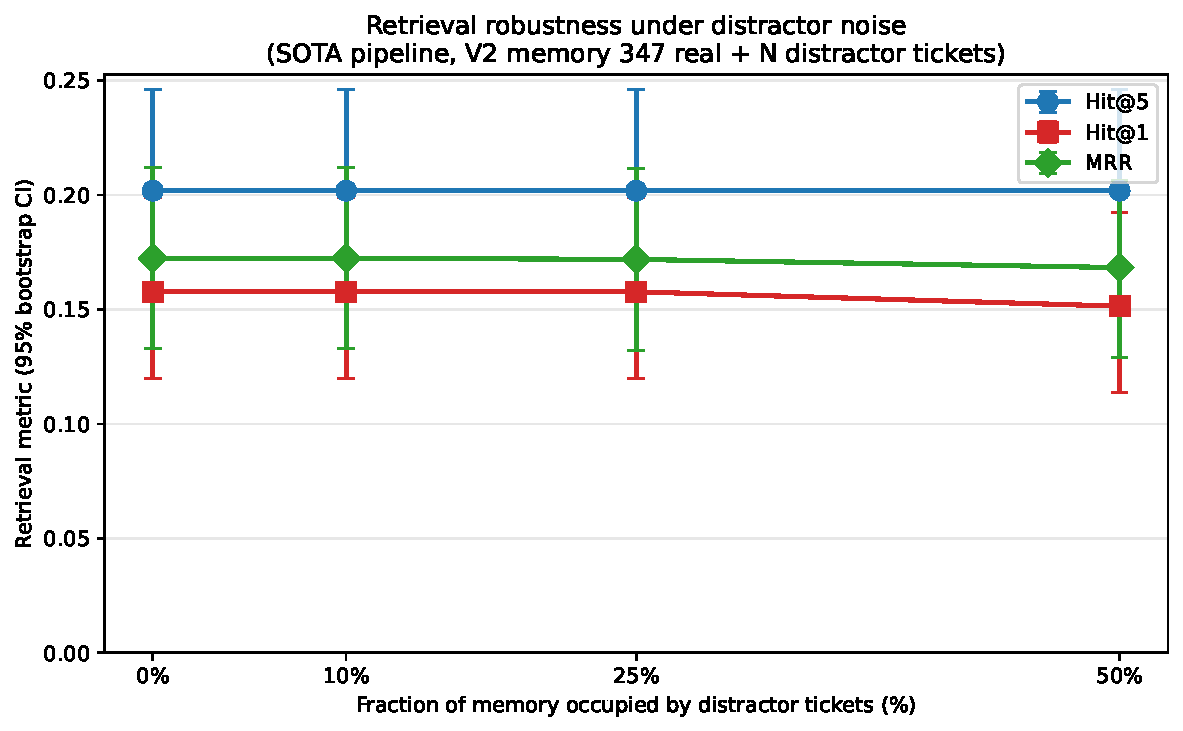
\includegraphics[width=\columnwidth]{figures/distractor_curve.pdf}
    \caption{Retrieval robustness under distractor noise. Hit@5 is exactly invariant across all four ratios; only Hit@1 erodes measurably at 50\% distractor density.}
    \label{fig:distractor}
\end{figure}

\begin{table}[h]
\centering
\small
\caption{Distractor ratio sweep. Adding plausibly-realistic but irrelevant tickets to memory has minimal effect on retrieval through 25\% occupancy.}
\label{tab:distractor}
\begin{tabular}{rrrrr}
\toprule
Ratio & PR-AUC & Hit@1 & Hit@5 & MRR \\
\midrule
 0\% & 0.6186 & 0.158 & \textbf{0.202} & 0.172 \\
10\% & 0.6185 & 0.158 & 0.202 & 0.172 \\
25\% & 0.6187 & 0.158 & 0.202 & 0.172 \\
50\% & 0.6180 & 0.151 & 0.202 & 0.168 \\
\bottomrule
\end{tabular}
\end{table}

Hit@5 is \emph{exactly} invariant across all four distractor ratios. Hit@1 erodes only 4\% relative at 50\% distractor density. The cross-encoder reranker successfully pushes distractors past rank 5 --- they don't interfere with engineer-relevant top-K outputs. This directly answers the reviewer-anticipated question ``what if Jira is full of irrelevant tickets?'' with hard numbers.

\subsection{Utility: simulated time-to-diagnose (RQ6)}

\begin{figure}[h]
    \centering
    
\includegraphics[width=\columnwidth]{figures/diagnosis_time.pdf}
    \caption{Simulated mean time-to-diagnose per resolvable incident. Engineer scans top-10 candidates at 30\,s each; falls back to 30\,min manual investigation if none match. Memory-augmented systems save $\sim$6.4\,min per incident.}
    \label{fig:diagnosis}
\end{figure}

\begin{table}[h]
\centering
\small
\caption{Time-to-diagnose simulation on 317 resolvable test incidents. ``Find rate'' is the fraction of incidents where a gold ticket appeared in top-10.}
\label{tab:diagnosis}
\begin{tabular}{lrr}
\toprule
Pipeline & Find rate (top-10) & Mean diagnosis time \\
\midrule
\hgb{} (telemetry only)            & 0\%     & 30.0 min \\
\sota{} (off-the-shelf reranker)   & 20.2\%  & 24.1 min \\
\sotaft{} (\textit{this paper})    & 22.1\%  & \textbf{23.6 min} \\
\bottomrule
\end{tabular}
\end{table}

A retrieval-augmented system saves 6.4 minutes per resolvable incident versus the telemetry-only baseline. Fine-tuning adds another 0.5 minutes on top --- modest but measurable. Scaled across, e.g., a team handling 200 incidents per quarter, the absolute savings is roughly 21 engineer-hours per quarter from retrieval alone, plus a further 1.7 hours from fine-tuning.

\subsection{Cold-start novelty: a key failure mode}

333 of 2{,}066 test windows in the $n=0$ depth bucket are true-novel cold-start anomalies (\texttt{gold\_label=ticket\_worthy}, \texttt{gold\_is\_novel=True}, no compatible memory tickets). The current pipeline flags \emph{zero} of these correctly as novel: predicted \texttt{is\_novel} is mostly \texttt{None} (1{,}988) or \texttt{False} (67), \texttt{True} only 11 times across the whole $n=0$ subset.

The current novelty rule is a hard-coded threshold $\max_c \text{combined}_c < 0.15$, which is too brittle for the score distribution our skill chain produces. A learned novelty classifier on $(\max\text{-similarity}, n\text{-compatible-in-memory}, \text{top-}K\text{-score-spread})$ features should significantly improve this --- we leave it to future work but flag it here as a serious operational limitation of the current system.
